\documentclass[12pt, a4paper]{article}

% ============================================================
% PACKAGES
% ============================================================
\usepackage[margin=1in]{geometry}
\usepackage{graphicx}
\usepackage{amsmath, amssymb}
\usepackage{booktabs}
\usepackage{float}
\usepackage{hyperref}
\usepackage{natbib}
\usepackage{setspace}
\usepackage{caption}
\usepackage{subcaption}
\usepackage{enumitem}
\usepackage{xcolor}
\usepackage{tabularx}
\usepackage{multirow}
\usepackage{array}

\hypersetup{
    colorlinks=true,
    linkcolor=blue,
    citecolor=blue,
    urlcolor=blue
}

\singlespacing

% ============================================================
% TITLE
% ============================================================
\title{\textbf{Hindi Fluency and Semantic Organization: \\Advanced Statistical Analysis} \\ \vspace{0.3cm} \large BRSM Project --- Report 2 (Final Submission)}
\author{
    Deban Kumar Shahi -- 2024201048 \\
    Md Fraz Uddin -- 2024201064 \\
    Suraj Lalwani -- 2024201071
}
\date{April 23, 2026}

\begin{document}
\maketitle

% ============================================================
% 1. INTRODUCTION
% ============================================================
\section{Introduction and Background}

Verbal Fluency Tests (VFTs) are a common tool in psychology and linguistics used to study how people organize and retrieve words from memory \citep{lezak2012neuropsychological}. In a typical VFT, participants are given a category (e.g., animals or colors) and asked to name as many items as they can within a time limit. By looking at \textbf{how quickly} participants produce words (measured through Inter-Response Times, or IRTs) and \textbf{how they arrange} words spatially, we can learn about how the mental dictionary is structured.

This report builds on our earlier Report~1, where we performed basic analyses such as $t$-tests and correlations. In this report, we go further by using more powerful methods: \textbf{ANOVA} (to compare multiple groups at once), \textbf{Linear Regression} (to see how one variable predicts another while controlling for other factors), \textbf{Generalized Linear Models} (to handle non-normal data like counts and response times), and \textbf{Bayesian Statistics} (to measure the strength of evidence for or against our hypotheses).

\subsection{What We Found in Report 1}

Report~1 analyzed 35 participants across four word categories and found:
\begin{itemize}[nosep]
    \item \textbf{Different categories, different word counts}: Participants produced the most words for Colours ($M = 13.36$, $SD = 3.41$) and the fewest for Body Parts ($M = 8.58$, $SD = 3.08$).
    \item \textbf{No timing difference between clusters}: The time gap between words within the same cluster ($M = 4732$ ms) was not very different from the gap when switching clusters ($M = 4923$ ms; $p = .400$).
    \item \textbf{A small spatial effect}: Words placed farther apart on the spatial grid had slightly faster retrieval times ($r = -0.117$, $p = .00024$).
    \item \textbf{Self-rated proficiency did not help predict performance}: Hindi proficiency scores did not significantly predict word count ($p = .376$) or retrieval speed ($p = .060$).
\end{itemize}

\subsection{Research Questions for Report 2}

In this report, we ask:
\begin{enumerate}[nosep]
    \item[\textbf{RQ1:}] Do the number of words produced differ across categories, and if so, which categories differ? (\textit{One-Way ANOVA with post-hoc tests})
    \item[\textbf{RQ2:}] Does retrieval speed depend on both the category and Hindi proficiency level? (\textit{Two-Way ANOVA})
    \item[\textbf{RQ3:}] Does the distance between consecutive words on the spatial grid predict how long it takes to retrieve the next word? (\textit{Multiple Regression})
    \item[\textbf{RQ4:}] Can we build better models for word counts and response times by using the right type of statistical model? (\textit{Generalized Linear Models})
    \item[\textbf{RQ5:}] How strong is the evidence for or against a relationship between Hindi proficiency and task performance? (\textit{Bayesian Analysis})
\end{enumerate}

\subsection{Dataset Description}

Our data comes from $N = 35$ participants who completed the Hindi Verbal Fluency Task (VFT) and the Spatial Arrangement Method (SpAM) task. Each participant worked on two or three categories: \textit{Animals} ($n = 35$), \textit{Foods} ($n = 35$), \textit{Colours} ($n = 11$), and \textit{Body Parts} ($n = 24$). The tasks were done online in a web browser, with participants typing their responses on a keyboard. In total, we collected 1,044 word responses and 1,040 spatial placements.

We also collected background information about each participant, including their self-rated Hindi and English proficiency (on a 1--5 scale), age, education level, first language, and home state.

% ============================================================
% 2. METHODS
% ============================================================
\section{Methods}

\subsection{Data Preprocessing}

We extracted three datasets from the raw JSON file using Python:
\begin{itemize}[nosep]
    \item \textbf{VFT data} (1,044 entries): Each word a participant typed, along with the category, the order it was typed in, and the time taken (IRT).
    \item \textbf{SpAM data} (1,040 entries): The final $(x, y)$ position where each word was placed on the 2D grid.
    \item \textbf{Demographics} (35 participants): Self-rated proficiency, age, education, and language background.
\end{itemize}

We calculated a \textbf{Hindi proficiency score} by averaging each participant's Hindi reading and writing ratings. To create High and Low proficiency groups for some analyses, we split participants at the median proficiency score. We excluded practice trials (the furniture category) from all analyses.

We also computed several new variables:
\begin{itemize}[nosep]
    \item \textbf{Semantic spread}: The average distance between all pairs of words on the SpAM grid, which tells us how spread out someone's word arrangement was.
    \item \textbf{Consecutive word distance}: The distance on the grid between each word and the word typed right before it.
    \item \textbf{Log-transformed IRT}: Since raw response times are heavily skewed (a few very slow responses pull the average up), we took the natural log of IRT to make the data more suitable for regression.
\end{itemize}

\subsection{Statistical Methods}

All analyses were done in Python using the \texttt{scipy}, \texttt{statsmodels}, and \texttt{pingouin} libraries. We used a significance level of $\alpha = 0.05$ for all tests.

\subsubsection{ANOVA (Analysis of Variance)}

\textbf{One-Way ANOVA} tests whether the average word count differs across the four categories. Before running it, we checked whether the spread of data was similar in each group (Levene's test). Since our group sizes were unequal, we also ran \textbf{Welch's ANOVA}, which works better in such cases. To find out \textit{which specific pairs} of categories differ, we used \textbf{Tukey's HSD} and \textbf{Games-Howell} post-hoc tests.

\textbf{Two-Way ANOVA} tested whether retrieval speed depends on category, proficiency level, or their combination (interaction).

\textbf{ANCOVA} tested category differences in retrieval speed while accounting for Hindi proficiency as a continuous variable (instead of splitting it into just ``high'' and ``low'').

We also checked whether the data met normality assumptions using Shapiro-Wilk tests, and where those assumptions were violated, we used the non-parametric \textbf{Kruskal-Wallis} test as a backup.

\subsubsection{Linear and Multiple Regression}

We built three regression models to predict $\log(\text{IRT})$, adding variables step by step:
\begin{enumerate}[nosep]
    \item \textbf{Model 1}: Uses only spatial distance as a predictor
    \item \textbf{Model 2}: Adds category (domain) as a control variable
    \item \textbf{Model 3}: Also adds word order (serial position) as a control
\end{enumerate}

This step-by-step approach helps us see whether spatial distance matters on its own, or only after we account for other factors. We compared models using $F$-tests and checked the quality of each model using residual plots and Q-Q plots.

\subsubsection{Generalized Linear Models (GLM)}

Standard regression assumes the outcome is a continuous, normally distributed number. But our data doesn't always fit this:
\begin{itemize}[nosep]
    \item \textbf{Word counts} are whole numbers (0, 1, 2, ...), so we used a \textbf{Poisson GLM}, which is designed for count data.
    \item \textbf{Response times (IRT)} are always positive and tend to be right-skewed, so we used a \textbf{Gamma GLM}, which handles this type of data well.
\end{itemize}

We checked for overdispersion (when the data is more spread out than the Poisson model expects) using the Pearson $\chi^2$/df ratio.

\subsubsection{Bayesian Statistics}

While standard tests give us $p$-values (the chance of seeing our data if there's truly no effect), Bayesian methods give us \textbf{Bayes Factors ($BF_{10}$)}, which tell us how much more likely the data is under the alternative hypothesis compared to the null. For example:
\begin{itemize}[nosep]
    \item $BF_{10} > 10$: Strong evidence that there IS an effect
    \item $BF_{10}$ around 1: We can't tell either way
    \item $BF_{10} < 0.1$: Strong evidence that there is NO effect
\end{itemize}

We used Bayesian $t$-tests, correlations, and model comparisons based on the BIC (Bayesian Information Criterion).


% ============================================================
% 3. RESULTS
% ============================================================
\section{Results}

\subsection{Analysis 1: One-Way ANOVA --- Word Production Across Categories}

First, we checked whether the variability in word counts was similar across categories. Levene's test confirmed this ($F(3, 101) = 0.578$, $p = .631$), so we can safely use ANOVA.

The ANOVA showed a \textbf{significant difference in word production across categories}:
\[
F(3, 101) = 4.050, \quad p = .009, \quad \eta_p^2 = .107
\]

The effect size ($\eta_p^2 = .107$) is a medium effect, meaning about 10.7\% of the difference in word counts is explained by which category was given.

Welch's ANOVA, which handles unequal group sizes better, confirmed this result: $F(3, 39.61) = 5.441$, $p = .003$.

\begin{table}[H]
\centering
\caption{Average word production for each category.}
\label{tab:domain_descriptives}
\begin{tabular}{lcccc}
\toprule
\textbf{Category} & \textbf{$n$} & \textbf{Mean} & \textbf{SD} & \textbf{95\% CI} \\
\midrule
Colours & 11 & 13.36 & 3.41 & [11.07, 15.66] \\
Animals & 35 & 10.43 & 4.60 & [8.85, 12.01] \\
Foods & 35 & 9.31 & 4.09 & [7.91, 10.72] \\
Body Parts & 24 & 8.58 & 3.08 & [7.28, 9.88] \\
\bottomrule
\end{tabular}
\end{table}

Next, we used \textbf{post-hoc tests} to find exactly which pairs of categories differ. Tukey's HSD (Table~\ref{tab:tukey}) revealed two significant differences:
\begin{itemize}[nosep]
    \item \textbf{Colours produced more words than Body Parts}: Difference $= 4.78$ words, $p = .008$, large effect (Hedges' $g = 1.47$).
    \item \textbf{Colours produced more words than Foods}: Difference $= 4.05$ words, $p = .022$, large effect (Hedges' $g = 1.01$).
\end{itemize}

No other pairs were significantly different. The Games-Howell test (which does not assume equal variances) confirmed both findings.

\textbf{Why does Colours stand out?} Colours is a smaller, more bounded category --- there are roughly 15--20 common color names, so participants can list most of them within the time limit. In contrast, Animals and Foods are much broader, with many sub-groups, making it harder to list everything.

\begin{table}[H]
\centering
\caption{Tukey HSD post-hoc comparisons between all pairs of categories.}
\label{tab:tukey}
\begin{tabular}{llcccc}
\toprule
\textbf{Group 1} & \textbf{Group 2} & \textbf{Mean Diff} & \textbf{$p_{adj}$} & \textbf{95\% CI} & \textbf{Sig.} \\
\midrule
Animals & Body Parts & $-1.85$ & .310 & [$-4.62$, $0.93$] & No \\
Animals & Colours & $2.94$ & .154 & [$-0.68$, $6.55$] & No \\
Animals & Foods & $-1.11$ & .651 & [$-3.62$, $1.39$] & No \\
Body Parts & Colours & $4.78$ & .008 & [$0.97$, $8.59$] & Yes \\
Body Parts & Foods & $0.73$ & .901 & [$-2.04$, $3.51$] & No \\
Colours & Foods & $-4.05$ & .022 & [$-7.67$, $-0.43$] & Yes \\
\bottomrule
\end{tabular}
\end{table}

\begin{figure}[H]
    \centering
    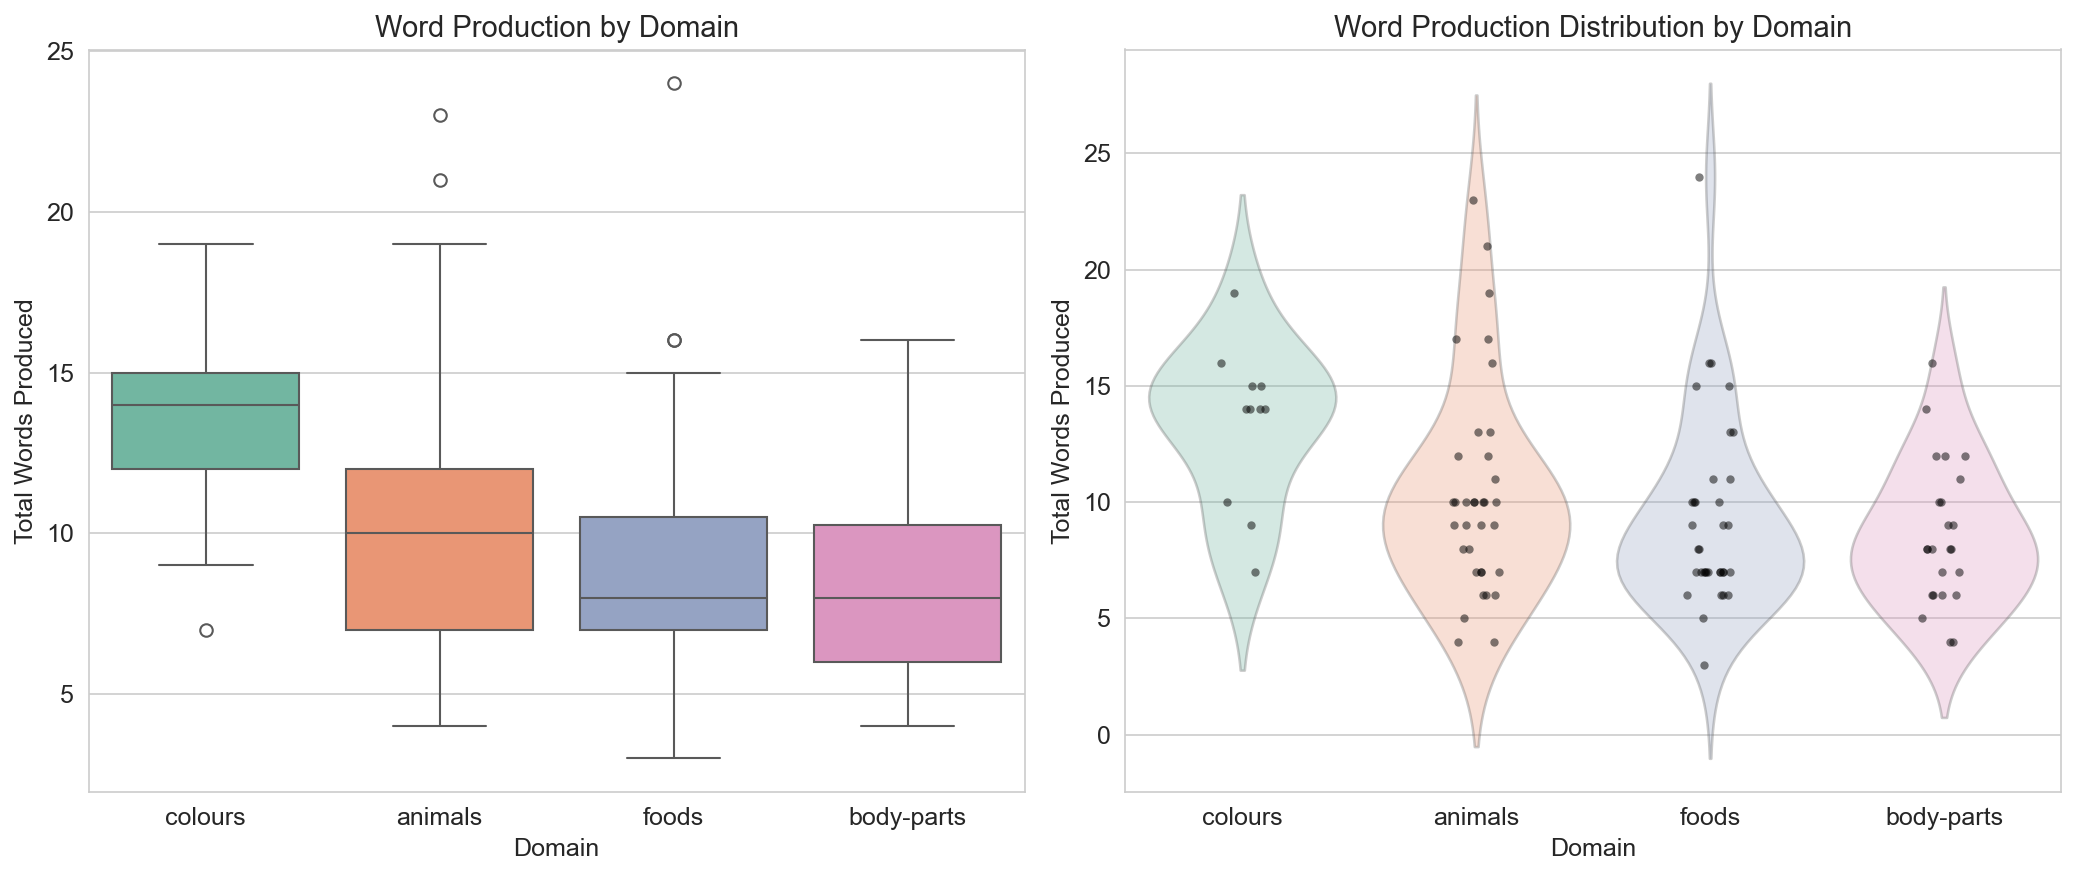
\includegraphics[width=0.95\textwidth]{figures/anova_word_production.png}
    \caption{Word production by category. Left: Box plots showing medians and ranges. Right: Violin plots with individual data points. Colours clearly stands out with higher word counts.}
    \label{fig:anova_words}
\end{figure}

\textbf{Normality check}: Shapiro-Wilk tests showed that the IRT data was not normally distributed for Foods ($W = 0.834$, $p < .001$) and Colours ($W = 0.740$, $p = .002$). So we also ran the \textbf{Kruskal-Wallis test}, a non-parametric alternative that doesn't assume normality. It was also significant ($H = 13.10$, $p = .004$), confirming our ANOVA results hold up.


\subsection{Analysis 2: Two-Way ANOVA --- Retrieval Speed by Category and Proficiency}

We tested whether retrieval speed (mean IRT) depends on the category, the participant's proficiency level, or a combination of both. We focused on Animals and Foods (the two categories with complete data, $n = 35$ each) and split participants into High and Low proficiency groups based on the median Hindi proficiency score.

\begin{table}[H]
\centering
\caption{Two-Way ANOVA results: Mean IRT by Category and Proficiency Group.}
\label{tab:twoway}
\begin{tabular}{lrrrrrr}
\toprule
\textbf{Source} & \textbf{SS} & \textbf{df} & \textbf{MS} & \textbf{$F$} & \textbf{$p$} & \textbf{$\eta_p^2$} \\
\midrule
Category & $7.38 \times 10^6$ & 1 & $7.38 \times 10^6$ & 0.930 & .338 & .014 \\
Proficiency & $2.39 \times 10^7$ & 1 & $2.39 \times 10^7$ & 3.016 & .087 & .044 \\
Category $\times$ Prof. & $1.91 \times 10^5$ & 1 & $1.91 \times 10^5$ & 0.024 & .877 & $<.001$ \\
Residual & $5.24 \times 10^8$ & 66 & $7.93 \times 10^6$ & & & \\
\bottomrule
\end{tabular}
\end{table}

\textbf{What we found}:
\begin{itemize}[nosep]
    \item \textbf{Category}: Not significant ($p = .338$). Animals and Foods don't differ much in retrieval speed.
    \item \textbf{Proficiency}: Close to significant ($p = .087$) but doesn't quite reach our threshold. Low-proficiency participants tend to be a bit slower.
    \item \textbf{Interaction}: Not significant ($p = .877$). The effect of proficiency on speed is the same for both categories --- the lines in the interaction plot are roughly parallel.
\end{itemize}

The proficiency effect is close but not significant here because we lost information by splitting a continuous score into just two groups. The ANCOVA (Analysis 3) handles this better.

\begin{figure}[H]
    \centering
    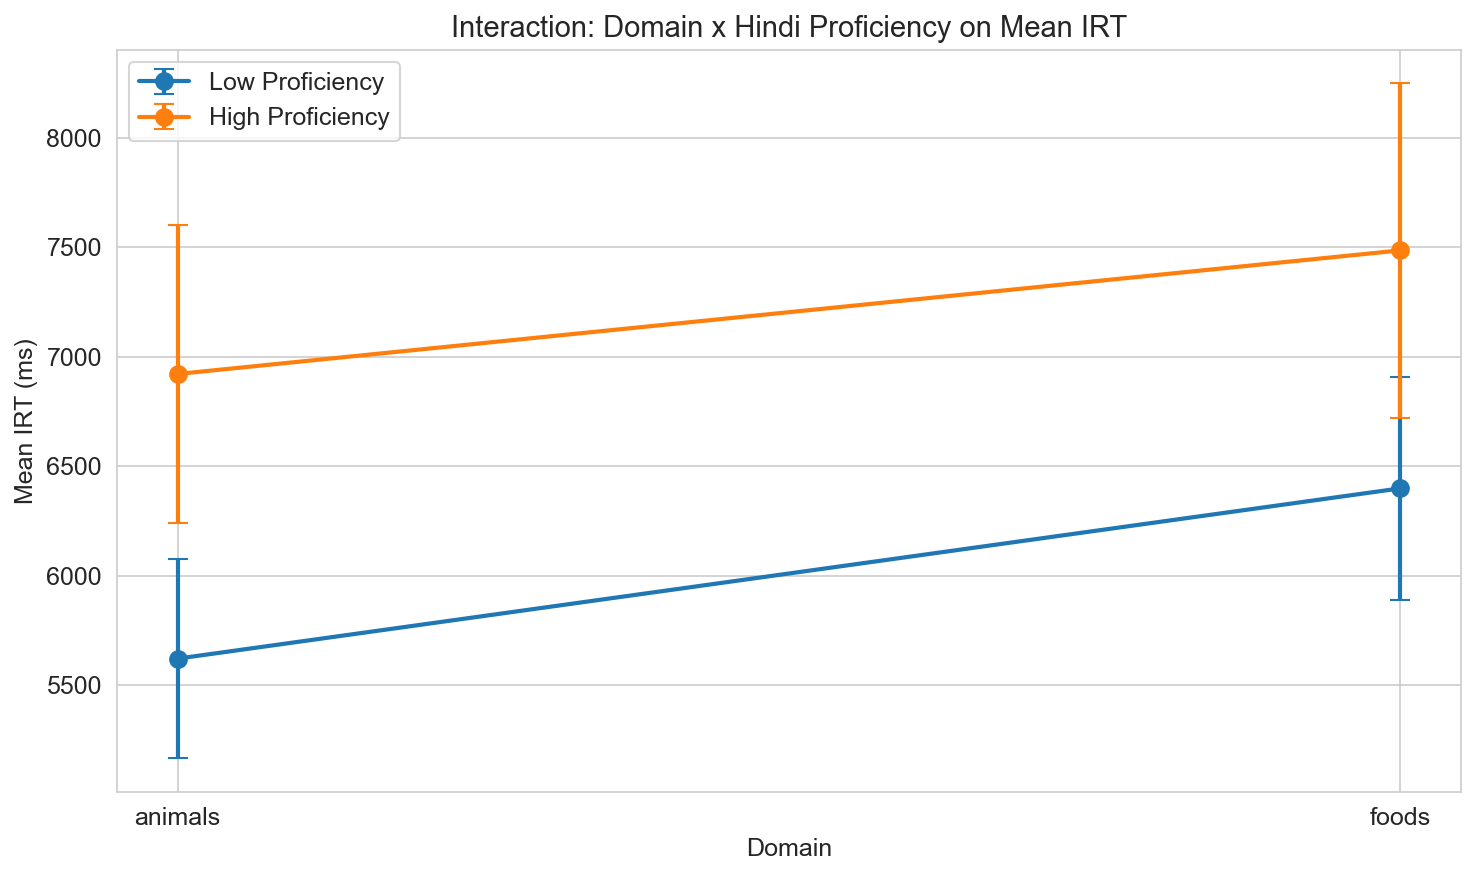
\includegraphics[width=0.7\textwidth]{figures/twoway_anova_interaction.png}
    \caption{Interaction plot: Mean IRT by Category and Proficiency Group. The nearly parallel lines show that proficiency affects retrieval speed similarly in both categories.}
    \label{fig:interaction}
\end{figure}

\subsection{Analysis 3: ANCOVA --- Retrieval Speed with Proficiency as a Covariate}

Instead of splitting proficiency into two groups, ANCOVA keeps it as a continuous number, which preserves more information and gives us more statistical power.

\begin{table}[H]
\centering
\caption{ANCOVA results: Mean IRT across categories, controlling for Hindi proficiency.}
\label{tab:ancova}
\begin{tabular}{lrrrrr}
\toprule
\textbf{Source} & \textbf{SS} & \textbf{df} & \textbf{$F$} & \textbf{$p$} & \textbf{$\eta_p^2$} \\
\midrule
Category & $6.94 \times 10^7$ & 3 & 3.279 & .024 & .090 \\
Hindi Proficiency & $5.37 \times 10^7$ & 1 & 7.603 & .007 & .071 \\
Residual & $7.06 \times 10^8$ & 100 & & & \\
\bottomrule
\end{tabular}
\end{table}

\textbf{This is one of the most important findings in this report:}

\begin{itemize}[nosep]
    \item \textbf{Category significantly predicts IRT} ($p = .024$), even after accounting for proficiency.
    \item \textbf{Hindi proficiency is now significant} ($p = .007$), explaining 7.1\% of the variation in retrieval speed. Higher proficiency is linked to faster word retrieval.
\end{itemize}

In Report~1, the link between proficiency and IRT was not significant ($p = .060$). The reason it was missed is that different categories have different average IRTs, and this category-level noise was hiding the true proficiency effect. Once ANCOVA removes the category effect, the proficiency--speed relationship becomes clear.


\subsection{Analysis 4: Linear Regression --- Does Spatial Distance Predict Retrieval Time?}

\subsubsection{Simple Regression (One Predictor)}

We first tested whether the spatial distance between two consecutive words on the SpAM grid predicts how long it took to retrieve the second word:
\[
\log(\text{IRT}) = 8.245 + 0.031 \times \text{SpatialDist}, \quad R^2 = .0001, \quad p = .750
\]

\textbf{Result}: Not significant at all. Spatial distance by itself does NOT predict retrieval time. This matches what Report~1 found.

But this doesn't mean there's no relationship --- the effect might be hidden by a confounding variable.

\subsubsection{Multiple Regression (Adding Controls)}

When we add \textbf{category} as a control variable, the picture changes completely:

\begin{table}[H]
\centering
\caption{Regression results after controlling for category.}
\label{tab:reg_model2}
\begin{tabular}{lrrrr}
\toprule
\textbf{Predictor} & \textbf{$\beta$} & \textbf{SE} & \textbf{$t$} & \textbf{$p$} \\
\midrule
Intercept & 8.200 & 0.046 & 178.19 & $<.001$ \\
Spatial Distance & 0.202 & 0.100 & 2.013 & .044 \\
Category: Body Parts & 0.212 & 0.066 & 3.236 & .001 \\
Category: Colours & $-0.296$ & 0.072 & $-4.123$ & $<.001$ \\
Category: Foods & 0.021 & 0.056 & 0.379 & .705 \\
\bottomrule
\end{tabular}
\end{table}

\textbf{Now spatial distance IS significant} ($\beta = 0.202$, $p = .044$). This means that, within the same category, words placed further apart on the grid do take longer to retrieve. The reason the simple regression missed this is that different categories have different spatial patterns AND different speeds. Category was acting as a confounding variable --- once we control for it, the true relationship appears.

Adding \textbf{word order (serial position)} as another control improved the model further:
\[
R^2 = .053, \quad \text{Model comparison: } F(4) = 12.35, \quad p < .001
\]

Word order was a significant negative predictor ($\beta = -0.017$, $p = .002$): later words are retrieved faster, likely because participants speed up as they exhaust items within a cluster.

\begin{figure}[H]
    \centering
    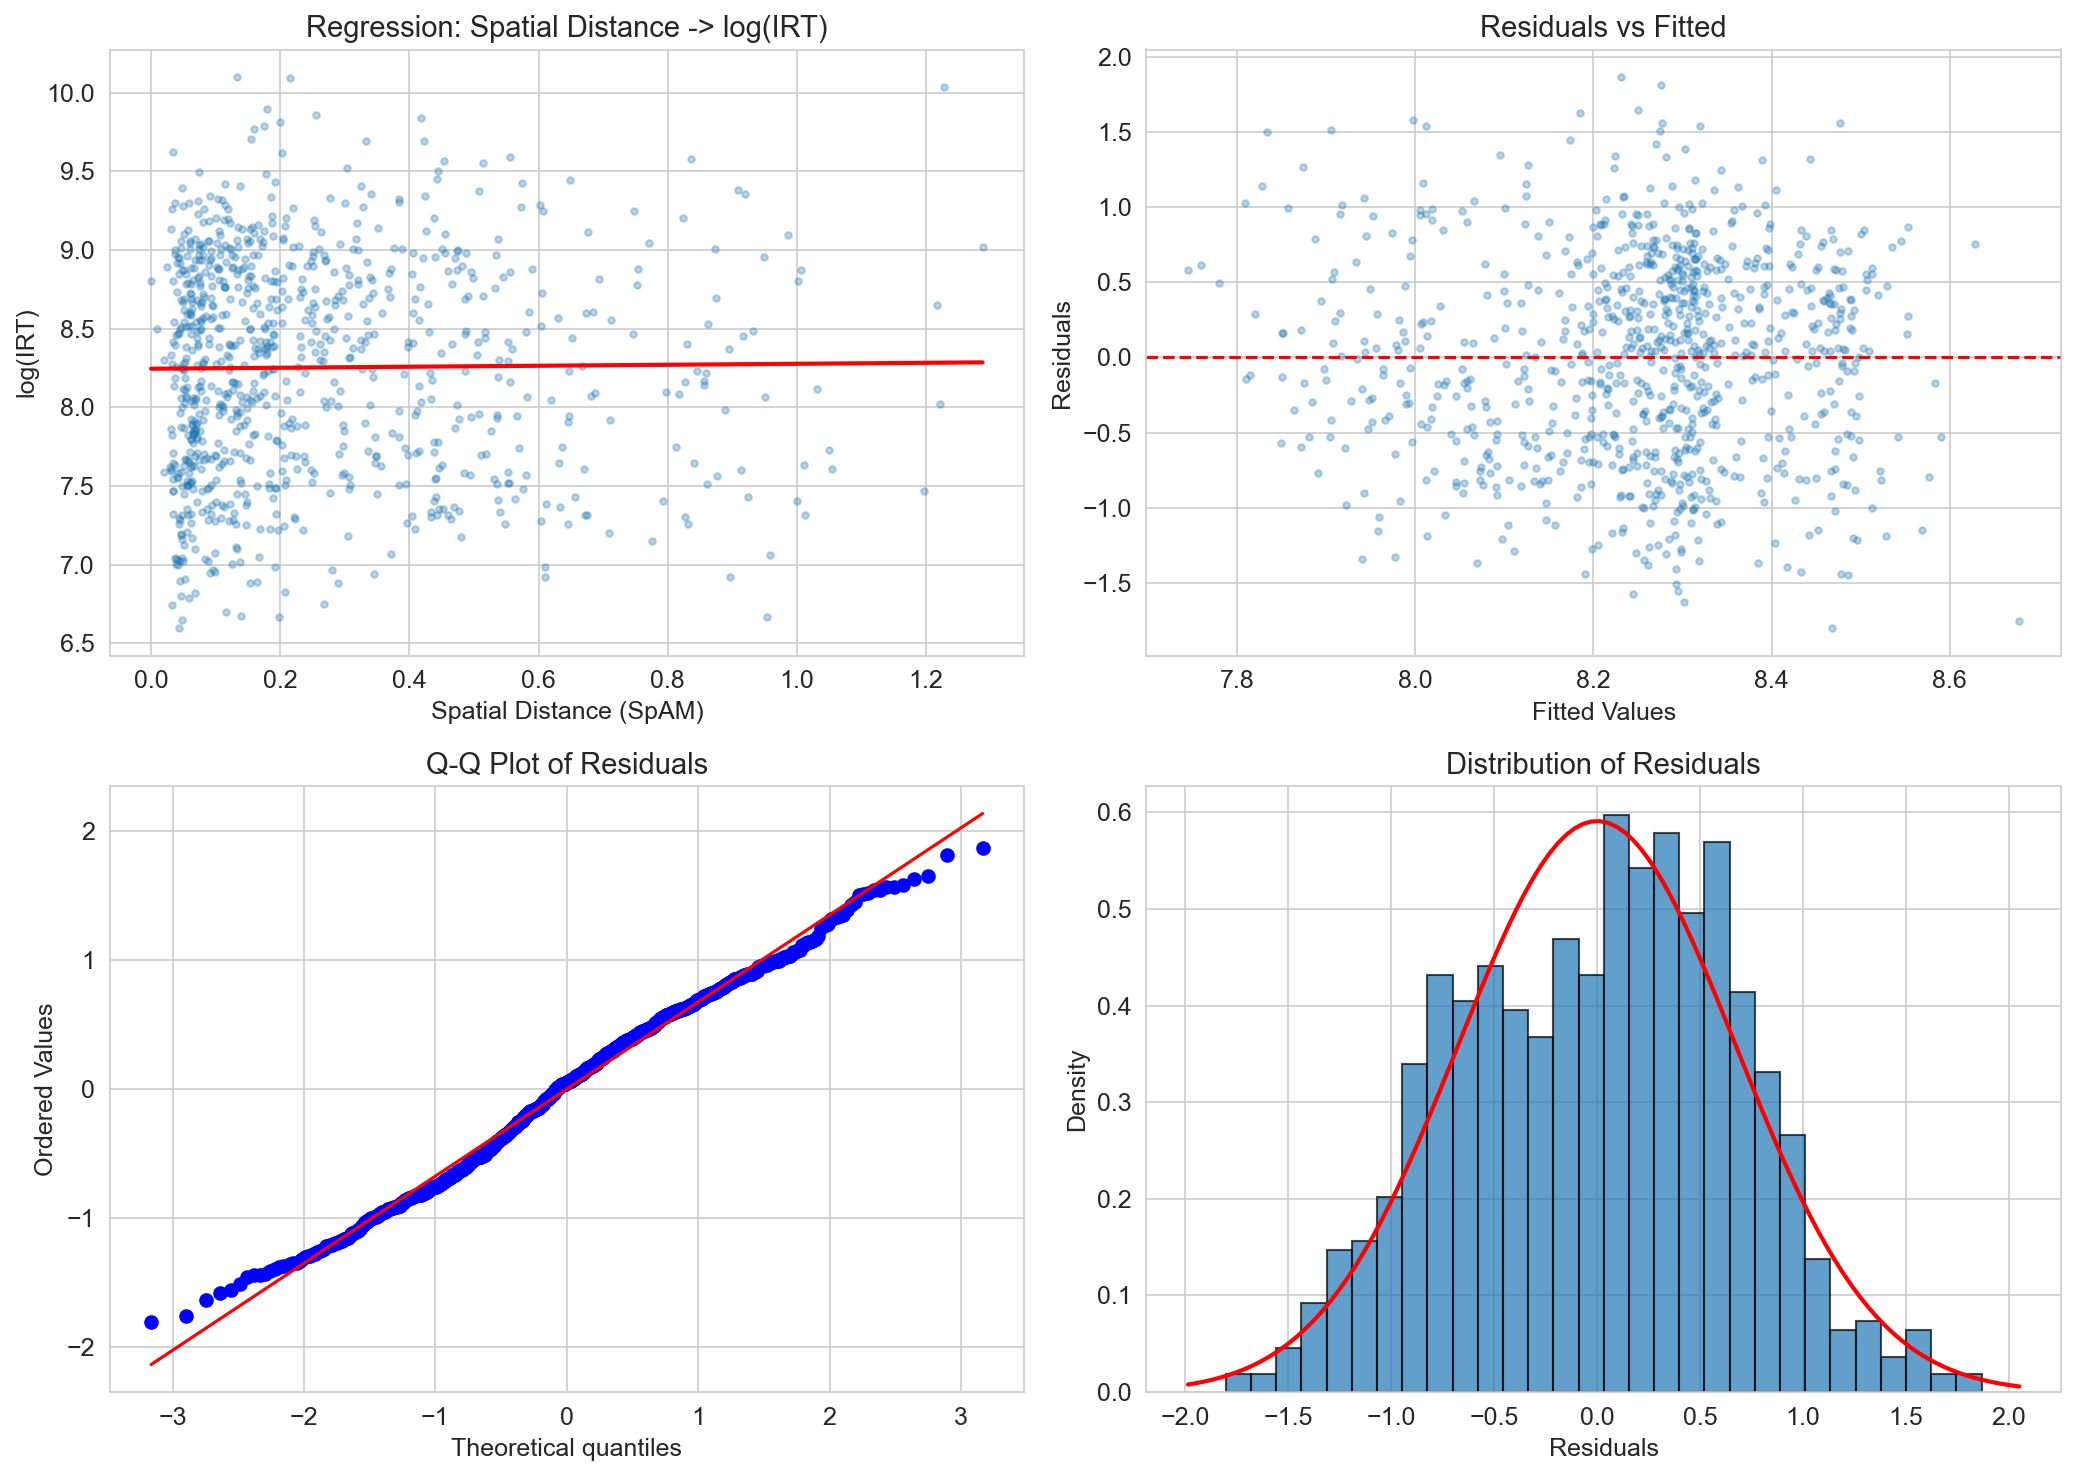
\includegraphics[width=\textwidth]{figures/regression_diagnostics.png}
    \caption{Regression diagnostics. Top-left: Scatter plot of spatial distance vs log(IRT) with regression line. Top-right: Residuals vs fitted values (no obvious pattern, which is good). Bottom-left: Q-Q plot showing residuals are roughly normal. Bottom-right: Histogram of residuals.}
    \label{fig:regression}
\end{figure}


\subsection{Analysis 5: Multiple Regression --- Predicting Total Word Count}

We tested whether proficiency ratings can predict how many words a participant produces:

\[
R^2 = .103, \quad F(5, 99) = 2.278, \quad p = .053
\]

\textbf{Key findings}:
\begin{itemize}[nosep]
    \item \textbf{Category} is a significant predictor ($F = 4.197$, $p = .008$): Some categories naturally produce more words than others.
    \item \textbf{Hindi proficiency}: Not significant ($p = .426$).
    \item \textbf{English proficiency}: Not significant ($p = .879$).
\end{itemize}

This confirms Report~1: how well you \textit{think} you know Hindi doesn't predict how many words you actually produce. Self-ratings may not capture the keyboard-typing skills and other practical factors that influence task performance.


\subsection{Analysis 6: Generalized Linear Models}

\subsubsection{Poisson GLM for Word Counts}

Word counts are integers (0, 1, 2, ...), so a model designed for count data (Poisson GLM) fits better than ordinary regression:

\begin{table}[H]
\centering
\caption{Poisson GLM results for predicting word counts.}
\label{tab:poisson}
\begin{tabular}{lrrrr}
\toprule
\textbf{Predictor} & \textbf{$\beta$} & \textbf{SE} & \textbf{$z$} & \textbf{$p$} \\
\midrule
Intercept & 2.349 & 0.158 & 14.899 & $<.001$ \\
Hindi Proficiency & $-0.016$ & 0.020 & $-0.800$ & .424 \\
English Proficiency & $-0.003$ & 0.022 & $-0.152$ & .879 \\
Category: Body Parts & $-0.213$ & 0.058 & $-3.660$ & $<.001$ \\
Category: Colours & 0.245 & 0.063 & 3.909 & $<.001$ \\
Category: Foods & $-0.114$ & 0.052 & $-2.183$ & .029 \\
\bottomrule
\end{tabular}
\end{table}

\textbf{How to read Poisson coefficients}: We exponentiate them to get multiplicative effects. For example:
\begin{itemize}[nosep]
    \item Colours vs Animals: $e^{0.245} = 1.28$, meaning Colours produces about \textbf{28\% more words} than Animals.
    \item Body Parts vs Animals: $e^{-0.213} = 0.81$, meaning Body Parts produces about \textbf{19\% fewer words}.
\end{itemize}

The dispersion parameter was $1.61$ (greater than 1), which means the data has more variability than a Poisson model expects (overdispersion). We also fitted a Negative Binomial GLM to handle this, and the results were the same.

\subsubsection{Gamma GLM for Retrieval Speed}

Since response times (IRT) are always positive and skewed to the right, a Gamma GLM is more appropriate than ordinary regression:

\begin{table}[H]
\centering
\caption{Gamma GLM results for predicting mean IRT.}
\label{tab:gamma}
\begin{tabular}{lrrrr}
\toprule
\textbf{Predictor} & \textbf{$\beta$} & \textbf{SE} & \textbf{$z$} & \textbf{$p$} \\
\midrule
Intercept & 9.139 & 0.274 & 33.367 & $<.001$ \\
Hindi Proficiency & $-0.091$ & 0.040 & $-2.249$ & .025 \\
Total Words & $-0.027$ & 0.013 & $-2.002$ & .045 \\
Category: Body Parts & 0.155 & 0.111 & 1.397 & .162 \\
Category: Colours & $-0.347$ & 0.129 & $-2.685$ & .007 \\
Category: Foods & 0.072 & 0.105 & 0.684 & .494 \\
\bottomrule
\end{tabular}
\end{table}

\textbf{Important findings}:
\begin{itemize}[nosep]
    \item \textbf{Hindi proficiency significantly predicts IRT} ($p = .025$): Each 1-point increase in proficiency reduces retrieval time by about 8.7\%. More proficient speakers retrieve words faster.
    \item \textbf{Word count also predicts IRT} ($p = .045$): Participants who produce more words also tend to be faster.
    \item \textbf{Colours is significantly faster} ($p = .007$): Colour words are retrieved about 29\% faster than animal words.
\end{itemize}

The Gamma GLM found the proficiency effect that ordinary regression missed, because it correctly accounts for the skewed, positive-only nature of response time data.

\subsubsection{Word-Level Gamma GLM}

At the individual word level, the Gamma GLM confirmed that later-typed words are retrieved faster:
\[
\beta_{\text{word\_order}} = -0.016, \quad z = -2.993, \quad p = .003
\]

\begin{figure}[H]
    \centering
    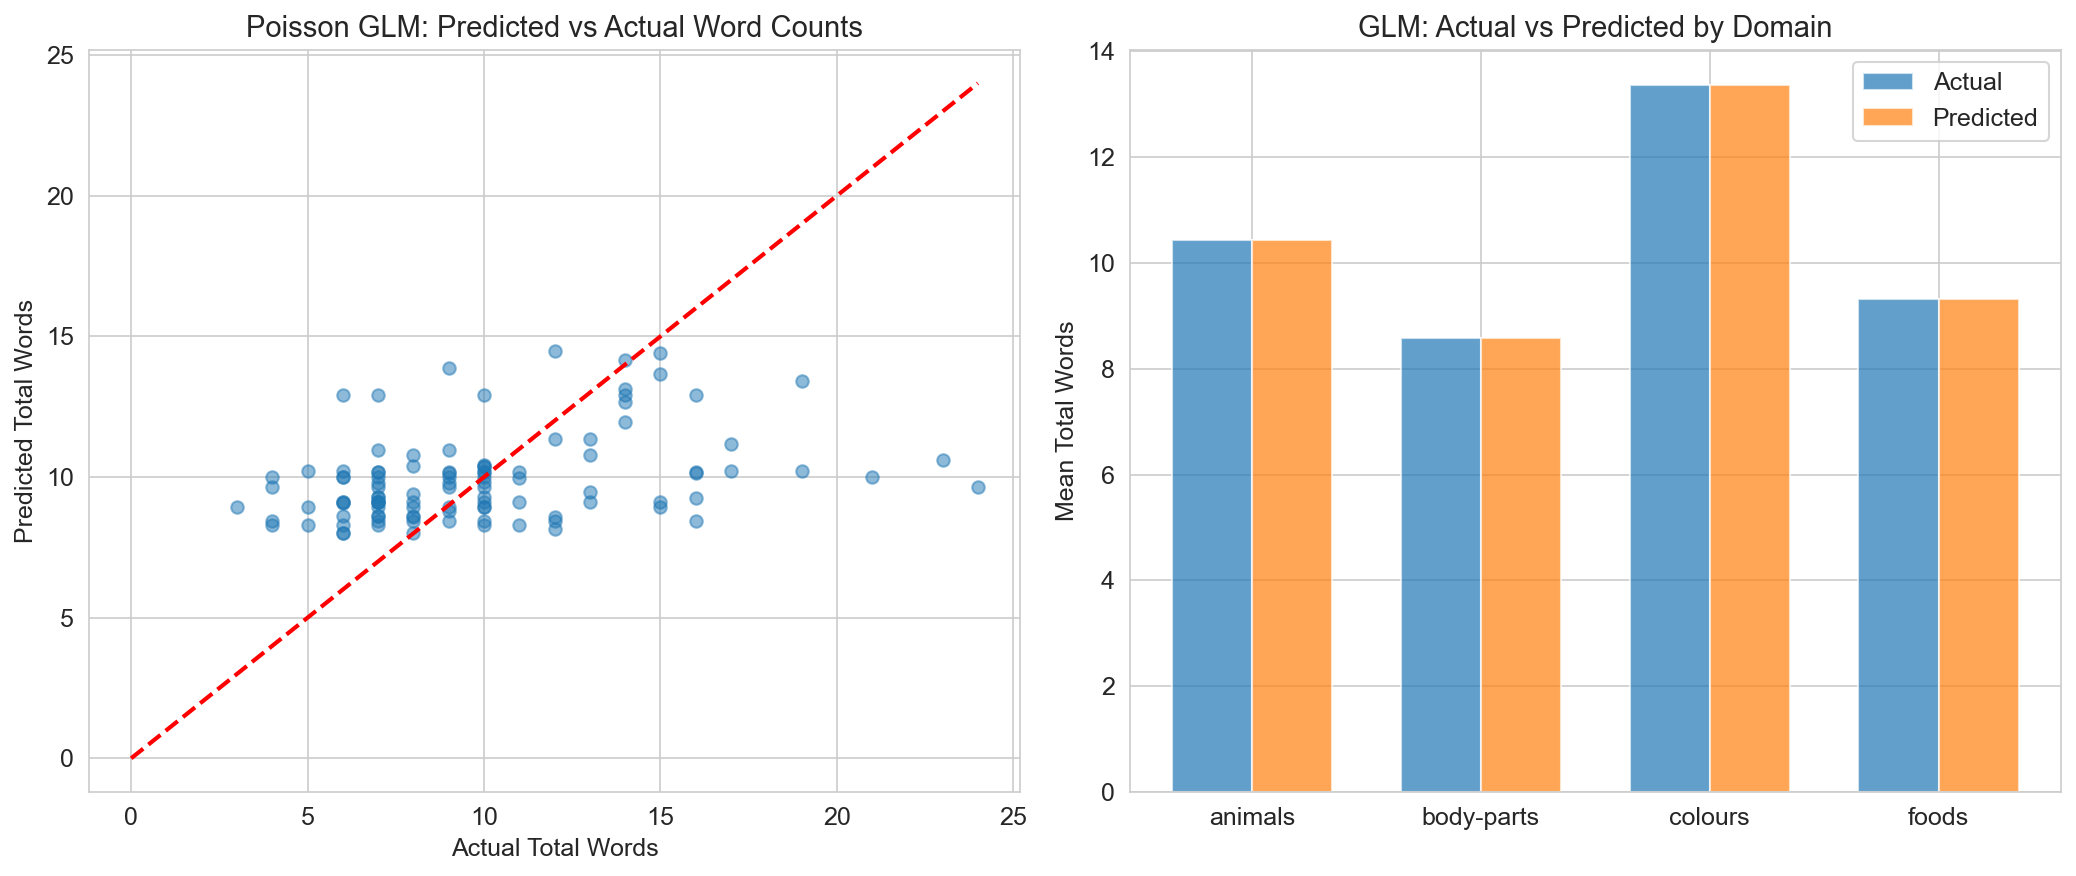
\includegraphics[width=0.95\textwidth]{figures/glm_results.png}
    \caption{Poisson GLM evaluation. Left: Predicted vs. actual word counts (points near the diagonal line mean good predictions). Right: Comparing actual and predicted averages for each category.}
    \label{fig:glm}
\end{figure}


\subsection{Analysis 7: Serial Position Effect}

We tested whether the position of a word in the sequence affects retrieval speed:
\[
\beta_{\text{word\_order}} = -0.017, \quad t = -3.179, \quad p = .002
\]

Each step forward in the sequence reduces $\log(\text{IRT})$ by 0.017, which translates to roughly a \textbf{1.7\% speedup per position}. By the 10th word, a participant is about 16\% faster than they were at the first word.

This ``speedup'' pattern makes sense: participants typically start with the most obvious words (which may take a moment to initiate), then rattle off related words quickly (within-cluster acceleration), and finally slow down again when they run out of easy words and need to switch to a new sub-group.

\begin{figure}[H]
    \centering
    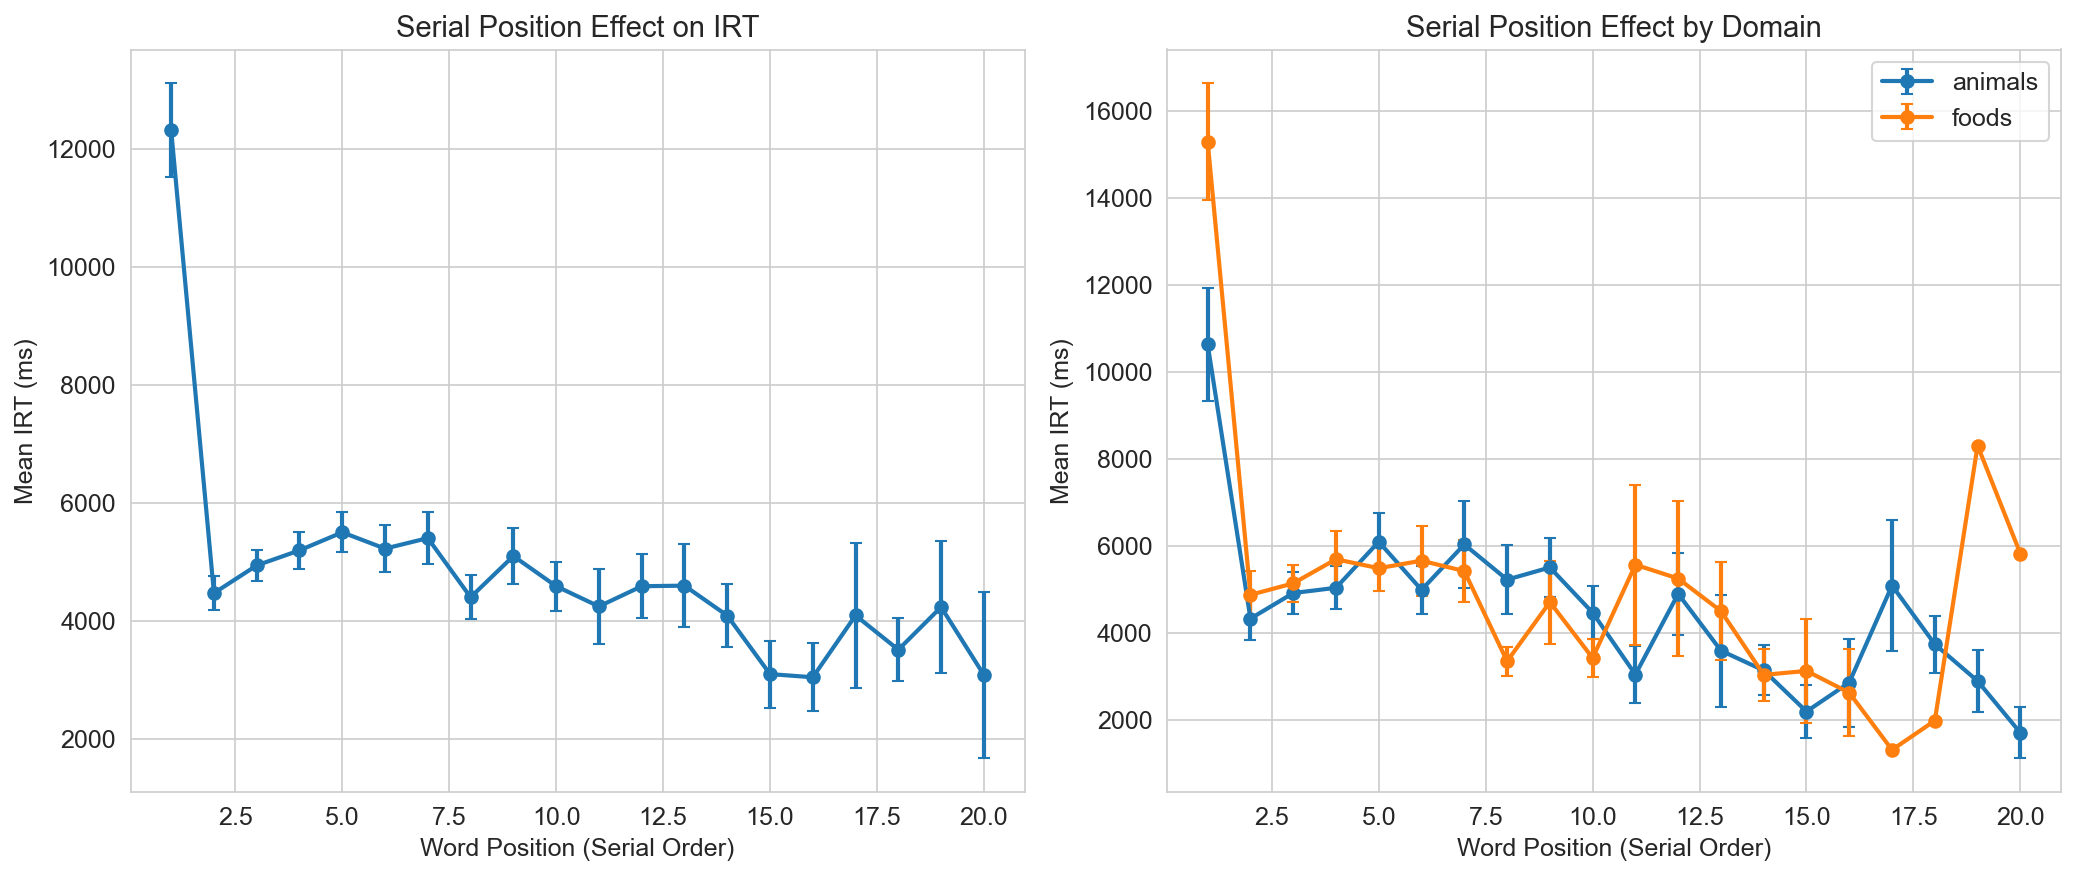
\includegraphics[width=0.95\textwidth]{figures/serial_position_effect.png}
    \caption{Serial position effect. Left: Mean IRT at each word position (averaged across all participants and categories). Right: The same pattern shown separately for Animals and Foods, with a visible slowdown after position 12--15.}
    \label{fig:serial}
\end{figure}


\subsection{Analysis 8: Bayesian Analysis}

\subsubsection{Bayesian $t$-test: Retrieval Speed by Proficiency Group}

The Bayesian $t$-test comparing mean IRT between High and Low proficiency groups gave $BF_{10} = 1.02$. This means the data is roughly equally likely under both hypotheses --- we can't tell from this test alone whether proficiency affects speed. This is consistent with the Two-Way ANOVA result ($p = .087$), where the effect was close but not definitive.

\subsubsection{Bayesian Correlation: Spatial Distance and IRT}

The Bayesian correlation between spatial distance and raw IRT gave $BF_{10} = 0.064$, which is \textbf{strong evidence for the null hypothesis}: there is no simple relationship between spatial distance and retrieval time when we don't control for category. This matches the frequentist result ($p = .750$).

\subsubsection{Bayesian Model Comparison}

We compared two models for predicting word counts:
\begin{itemize}[nosep]
    \item \textbf{Null model}: Just predicts the overall average (no predictors)
    \item \textbf{Full model}: Uses Hindi proficiency and category as predictors
\end{itemize}

Results:
\begin{itemize}[nosep]
    \item Null Model BIC: 602.02
    \item Full Model BIC: 606.81
    \item $BF_{10} \approx 0.091$
\end{itemize}

A $BF_{10}$ of 0.091 means there is \textbf{strong evidence that proficiency does NOT help predict word counts}. The Bayesian analysis agrees with the frequentist result: knowing someone's Hindi proficiency doesn't help us predict how many words they will produce.

\textbf{The Bayesian takeaway}: Proficiency affects \textit{how fast} you retrieve words (speed), but NOT \textit{how many} words you produce (volume). These are two partially separate processes.


\subsection{Correlation Structure}

\begin{figure}[H]
    \centering
    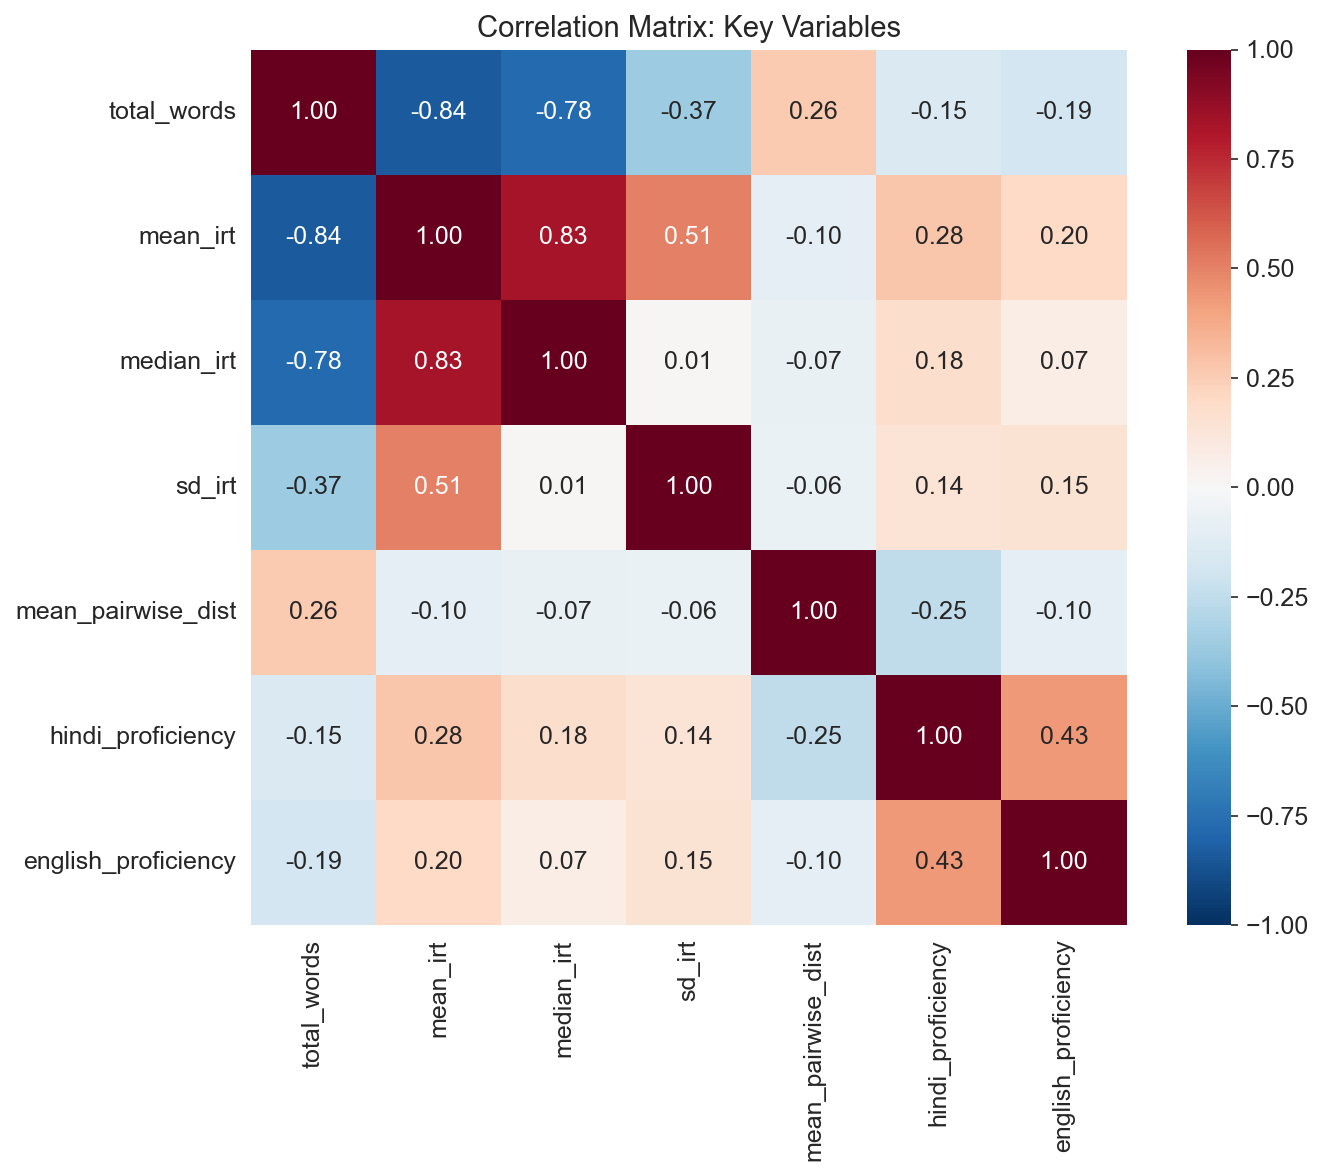
\includegraphics[width=0.75\textwidth]{figures/correlation_heatmap.png}
    \caption{Correlation matrix showing relationships between key variables. Total words and mean IRT have a moderate negative correlation (more words = faster retrieval). Proficiency ratings show weak connections to actual task performance.}
    \label{fig:corr}
\end{figure}

\begin{figure}[H]
    \centering
    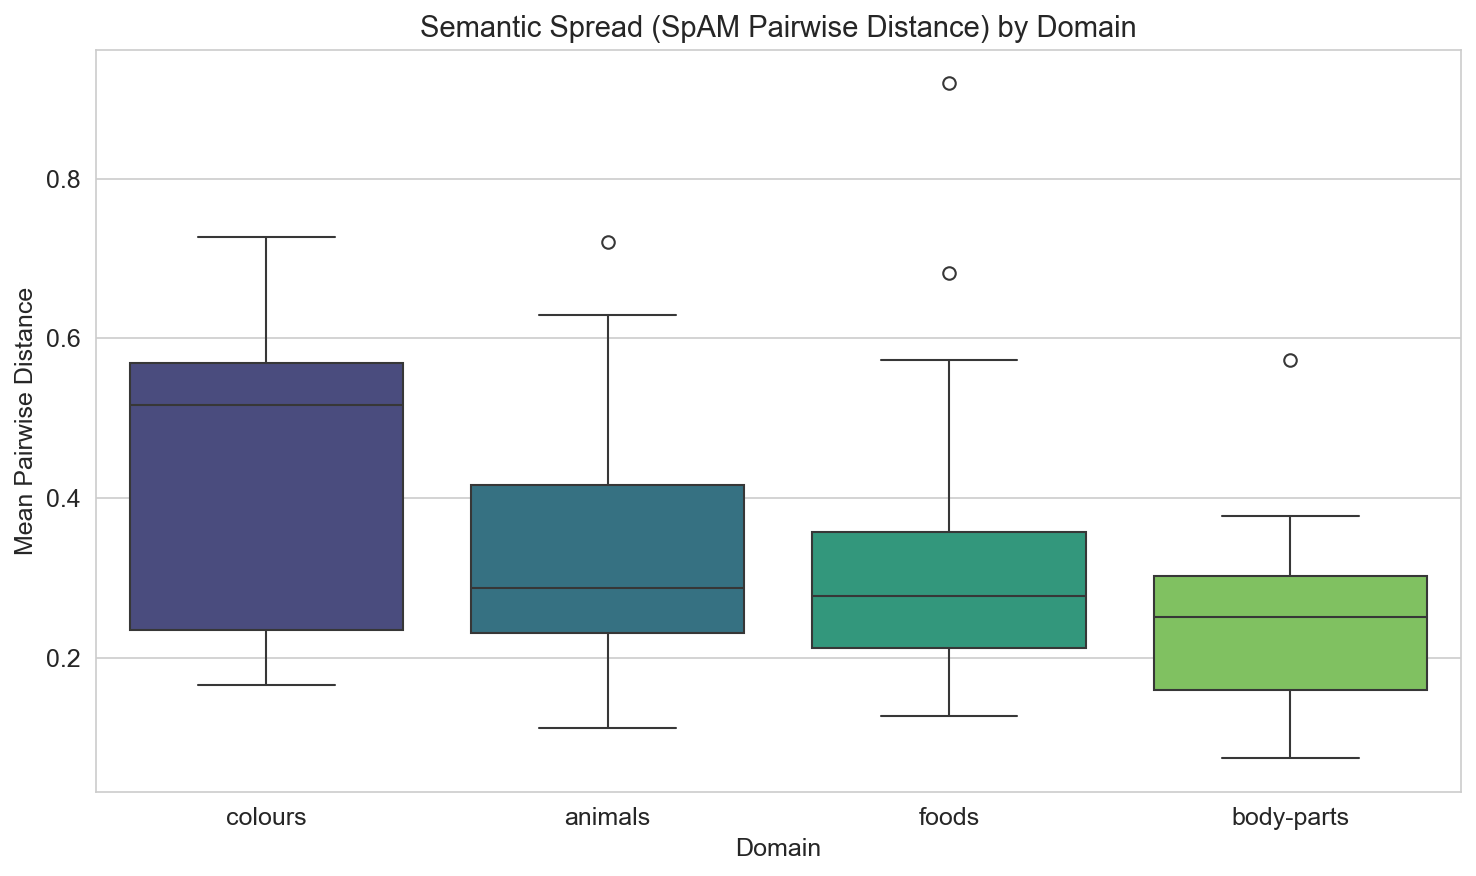
\includegraphics[width=0.75\textwidth]{figures/spam_spread_by_domain.png}
    \caption{How spread out participants' word arrangements were on the SpAM grid, shown by category.}
    \label{fig:spam_spread}
\end{figure}


% ============================================================
% 4. DISCUSSION AND CONCLUSIONS
% ============================================================
\section{Discussion and Conclusions}

\subsection{Summary of Findings}

This report used ANOVA, regression, GLMs, and Bayesian methods to investigate how Hindi speakers organize and retrieve words from their mental dictionary. Here are the key takeaways:

\begin{enumerate}
    \item \textbf{Category matters for word production.} The ANOVA ($p = .009$) showed that participants produced significantly more words for Colours than for Body Parts or Foods. This is likely because Colours is a smaller, more contained category where people can list most items within the time limit.

    \item \textbf{Proficiency predicts retrieval speed --- but you need the right analysis.} Report~1 found that proficiency was not significant ($p = .060$). However, the ANCOVA ($p = .007$) showed that this was a false negative: the category effect was hiding the true proficiency effect. The Gamma GLM also confirmed this ($p = .025$). Meanwhile, the Bayesian analysis ($BF_{10} = 0.091$) showed strong evidence that proficiency does NOT predict word \textit{count}. So proficiency affects \textit{speed} but not \textit{quantity}.

    \item \textbf{Spatial distance does predict retrieval time --- but only after controlling for category.} The simple correlation ($p = .750$) showed nothing, but the multiple regression ($p = .044$) revealed the hidden effect. Words placed further apart on the grid take longer to produce in sequence, consistent with the idea that people retrieve words in semantic clusters \citep{troyer1997clustering}.

    \item \textbf{There is a serial position effect.} Later words are retrieved faster ($p = .002$), reflecting within-cluster speedup before the participant needs to switch to a new sub-category.

    \item \textbf{Choosing the right statistical model matters.} The Gamma GLM found significant effects that ordinary regression missed, because it properly handles the skewed nature of response time data. The Poisson GLM is more appropriate for word counts than treating them as continuous numbers.
\end{enumerate}

\subsection{What These Methods Add Over Report 1}

\begin{itemize}[nosep]
    \item \textbf{ANOVA with post-hoc tests} told us \textit{which} categories differ, not just that ``some difference exists.''
    \item \textbf{ANCOVA} found a real proficiency effect ($p = .007$) that was hidden in Report~1's simpler analysis ($p = .060$).
    \item \textbf{Multiple regression} revealed that category was confounding the spatial distance--IRT relationship, and that serial position is also important.
    \item \textbf{GLMs} gave us more accurate models by matching the statistical model to the actual distribution of the data.
    \item \textbf{Bayesian analysis} confirmed our findings from a different angle and provided clear quantification of the evidence.
\end{itemize}

\subsection{Limitations}

\begin{itemize}[nosep]
    \item \textbf{Unequal group sizes}: Colours had only 11 participants while Animals and Foods had 35 each, which reduces the reliability of comparisons involving Colours.
    \item \textbf{Typing speed as a confound}: IRT measures both thinking time and typing time. A slow typist might appear to have slow retrieval even if they're thinking quickly. Future studies could use voice recording instead.
    \item \textbf{Self-reported proficiency is imprecise}: Asking people to rate their own Hindi ability on a 1--5 scale is a rough measurement. Standardized language tests would be more accurate.
    \item \textbf{Full Bayesian modeling was not possible}: Due to compiler issues on Windows, we could not run PyMC for full posterior estimation. We used BIC-based approximations instead, which are a reasonable but less detailed alternative.
\end{itemize}

\subsection{Future Directions}

\begin{itemize}[nosep]
    \item \textbf{Mixed-effects models}: These would better handle the fact that each participant contributes multiple observations (words nested within participants).
    \item \textbf{Automatic cluster detection}: Instead of manually defining clusters, algorithms like DBSCAN could identify semantic groups from the SpAM coordinates automatically.
    \item \textbf{Voice-based testing}: Recording spoken responses instead of typing would remove the keyboard confound.
    \item \textbf{Comparing Hindi and English}: Testing the same participants in both languages would reveal how bilingual speakers organize different languages in their mind.
\end{itemize}


% ============================================================
% TEAM CONTRIBUTIONS
% ============================================================
\section{Team Contributions}

\begin{itemize}[nosep]
    \item \textbf{Deban Kumar Shahi (2024201048)}: Led the ANOVA and regression analyses. Managed assumption checking, model diagnostics, and statistical methodology decisions.
    \item \textbf{Md Fraz Uddin (2024201064)}: Built the Python analysis pipeline, created all figures, ran GLM and Bayesian analyses, and wrote the report.
    \item \textbf{Suraj Lalwani (2024201071)}: Extracted and cleaned data from the JSON file, computed SpAM-based metrics (pairwise distances, consecutive word distances), and handled data preprocessing.
\end{itemize}


% ============================================================
% REFERENCES
% ============================================================
\bibliographystyle{apalike}
\begin{thebibliography}{9}

\bibitem[Dautriche et~al., 2016]{dautriche2016wordform}
Dautriche, I., Mahowald, K., Gibson, E., \& Piantadosi, S.~T. (2016).
\newblock Wordform similarity increases with semantic similarity: An analysis of 100 languages.
\newblock \textit{Cognitive Science}, 41, 2149--2169.

\bibitem[Jeffreys, 1961]{jeffreys1961theory}
Jeffreys, H. (1961).
\newblock \textit{Theory of Probability}. Oxford University Press.

\bibitem[Koch et~al., 2016]{koch2016spatial}
Koch, G.~E., Paynter, C.~A., \& Glisky, E.~L. (2016).
\newblock The spatial arrangement method of measuring similarity.
\newblock \textit{Behavior Research Methods}, 48, 442--456.

\bibitem[Lezak et~al., 2012]{lezak2012neuropsychological}
Lezak, M.~D., Howieson, D.~B., Bigler, E.~D., \& Tranel, D. (2012).
\newblock \textit{Neuropsychological Assessment} (5th ed.). Oxford University Press.

\bibitem[Troyer et~al., 1997]{troyer1997clustering}
Troyer, A.~K., Moscovitch, M., \& Winocur, G. (1997).
\newblock Clustering and switching as two components of verbal fluency: Evidence from younger and older healthy adults.
\newblock \textit{Neuropsychology}, 11(1), 138--146.

\bibitem[Preprint, 2024]{semantic_bilingual}
Semantic Modeling in Bilingual Lexicons. Pre-Print Archive.
\newblock \url{https://osf.io/preprints/psyarxiv/2bazx_v1}

\end{thebibliography}

\vspace{0.5cm}
\noindent\textbf{GitHub Repository}: \url{https://github.com/fraz-uddin07/BRSM_GRP_52}

\end{document}
